\documentclass[11pt]{article}
\usepackage{fullpage}
\usepackage{graphicx}
\usepackage{tikz}
\usepackage{hyperref}

\title{CS63 Spring 2017\\Lab 7: Neural Networks}
\author{Cindy Li, Grace Zhang}

\begin{document}

\maketitle

\section{XOR}

With random seed 24
our network achieved 100\% accuracy on the XOR data set after 10000
training epochs.
The resulting neural network is shown in the following diagram.

\begin{center}
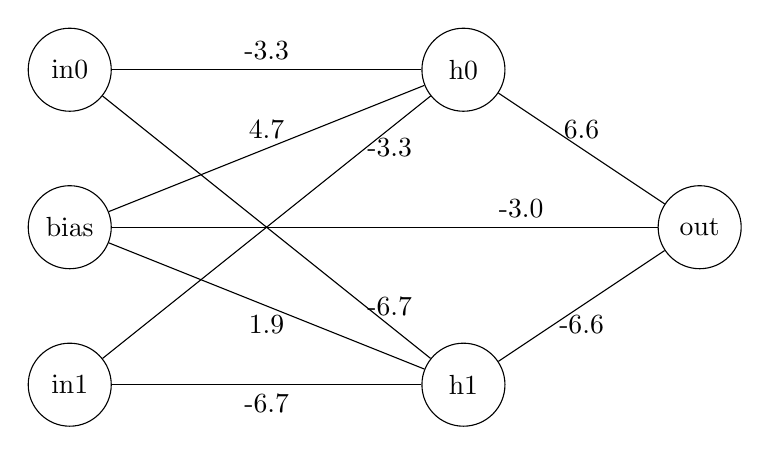
\begin{tikzpicture}
\tikzstyle{neuron}=[draw, circle, minimum size=30pt]

\draw (0,2) node[neuron] (bias) {bias};
\draw (0,4) node[neuron] (in0) {in0};
\draw (0,0) node[neuron] (in1) {in1};
\draw (5,4) node[neuron] (h0) {h0};
\draw (5,0) node[neuron] (h1) {h1};
\draw (8,2) node[neuron] (out) {out};

\draw (in0) edge node[above] {-3.3} (h0);
\draw (in0) edge node[very near end, above] {-6.7} (h1);
\draw (in1) edge node[very near end, below] {-3.3} (h0);
\draw (in1) edge node[below] {-6.7} (h1);
\draw (h0) edge node[above] {6.6} (out);
\draw (h1) edge node[below] {-6.6} (out);
\draw (bias) edge node[above] {4.7} (h0);
\draw (bias) edge node[below] {1.9} (h1);
\draw (bias) edge node[near end, above] {-3.0} (out);
\end{tikzpicture}
\end{center}

Looking at our truth tables:
\begin{center}
\begin{tabular}{ c c c c }
 in0 & in1 & h0 & h1 \\
  1 & 1 & 0 & 0\\
  0 & 1 & 1 & 0\\
  1 & 0 & 1 & 0\\
  0 & 0 & 1 & 1,
\end{tabular}
\end{center}

we can say that h0 represents the NAND gate while h1 represents the NOR gate. \\

Together, they are equivalent to the boolean function h0 AND (NOT h1):

\begin{center}

\begin{tabular}{ c c c}
 h0 & h1 & out\\
  1 & 1 & 0 \\
  0 & 1 & 0 \\
  1 & 0 & 1 \\
  0 & 0 & 0.
\end{tabular}
\end{center}


\section{Keras}

Here is how we achieved 97.88\%
accuracy on the MNIST handwritten digit data set.

\subsection{Parameters}

\begin{itemize}
 \item hidden layer activation: \texttt{relu}
 \item output layer activation: \texttt{softmax}
 \item optimizer=\texttt{Adam}
 \item loss=\texttt{mean\_squared\_error}
\end{itemize}

\subsection{Process}


First, we tried changing the number of epochs. Changing the value from 10 to 12 led to a 10\% increase in accuracy,
but a change from 12 to 20 epochs showed negligible results, so we decided to keep this number at 12. \\
Next, we played around with the number of hidden layers. Adding a hidden layer drastically decreased the performance
so we stuck to two hidden layers.
Afterwards, we played around with the other available activations. We found that changing one of the sigmoid activations
to relu resulted in an accuracy of 87.73\%. We changed the other sigmoid to a softmax activation according to Bryce's suggestion
in the lab write-up, resulting in an 89.47\% accuracy. \\
Finally, we changed our optimizer to Adam and kept our loss as mean\_squared\_error after playing around with a few. Some of the other optimizers we tried included the default SGD, RMSprop, and Adagrad. Some of the other loss functions we tried included squared\_hinge and poisson. \\
\url{https://keras.io/losses/} \url{https://keras.io/optimizers/}

\subsection{Explanation}
When using the ReLU activation function and the input is positive, the derivative is just 1, so there isn't the sqeezing effect you get on backpropagated errors like from the sigmoid function.

Softmax acts similarly to the sigmoid function, but normalizes the outputs so they are equivalent to a probability distribution, which tells you the probability that any of the classes are true. \\
\url{https://github.com/Kulbear/deep-learning-nano-foundation/wiki/ReLU-and-Softmax-Activation-Functions} \\

Adam maintains a per-parameter learning rate instead of a single learning rate (alpha) for all weight updates. This improves performance on data sets with sparse gradients. These per-parameter learning rates are adapted based on the average of recent gradients, so this algorithm can do well on online and noisy problems. \\
\url{https://machinelearningmastery.com/adam-optimization-algorithm-for-deep-learning/}


\end{document}
